\section{Ziel}
In diesem Versuch soll die effektive Masse der Leitungselektronen von n-dotiertem Galliumarsenid mithilfe des Faraday-Effekts bestimmt werden.

\section{Theorie}
\label{sec:Theorie}

\subsection{Halbleiter}


\subsection{Effektive Masse}
Die effektive Masse wird eingeführt, damit Elektronen wie freie Ladungsträger behandelt werden können. Im Kristall erfahren Elektronen ein Potential. In einem äußeren elektrischen Feld ändert sich deswegen nicht nur die kinetische Energie des Elektrons, sondern auch die potentielle. Bei der effektiven Masse ist das Potential berücksichtigt. \cite{demtroeder}

Die effektive Masse von Elektronen im Leitungsband bzw. von Löchern im Valenzband (\cite{demtroeder}) ist gegeben durch
\begin{equation*}
    m_\text{eff} = \hbar^2 \cdot \left( \frac{d^2 E}{dk_i \, dk_j} \right)^{-1}.
\end{equation*}
Die effektive Masse hat Tensorcharakter und gibt die inverse Krümmung der Dispersionsrelation $E(k)$ an. \cite{demtroeder}

\subsection{Faraday-Effekt}
Die Polarisationsebene von linear polarisiertem Licht in einem Medium wird gedreht, wenn das Licht parallel zu einem Magnetfeld durch das Material läuft. \cite{heintze}
Eine schematische Darstellung des Faraday-Effekts ist in Abb. \ref{fig:FaradayEffekt} zu sehen.
%Optisch inaktive Materie dreht beim Anlegen eines äußeren Magnetfeldes die Polarisationsebene des Lichts, das parallel zur Magnetfeldrichtung einfällt. \cite{V46}

Damit der Kristall die Polarisationsebene des linear polarisierten Lichts bei der Transmission drehen kann (zirkulare Doppelbrechung), muss die Phasengeschwindigkeit für links- und rechtszirkular polarisiertes Licht in dem Medium verschieden sein. Das bedeutet, dass die Brechungsindizes verschieden sind. \cite{V46}

Die Faraday-Rotation wird durch folgende Formel (\cite{V46}) berechnet
\begin{equation}
    \theta_\text{frei} = \frac{{e_0}^3}{8 \, \pi^2 \, \epsilon_0 \, c^3 \, {m_\text{eff}}^2} \frac{N \, B}{n} \lambda^2 = \frac{\theta}{L},
    \label{eq:theta}
\end{equation}
wobei $e_0$ die Elementarladung ist, $\epsilon_0$ die elektrische Feldkonstante, $c$ die Vakuum-Lichtgeschwindigkeit, $m_\text{eff}$ die effektive Masse, $N$ die Donatorenkonzentration, $B$ die Magnetfeldstärke, $n$ der Brechungsindex, $L$ die Probendicke und $\lambda$ die Wellenlänge.
Die Einheit der Faraday-Rotation ist $rad/m$.

\begin{figure}
    \centering
    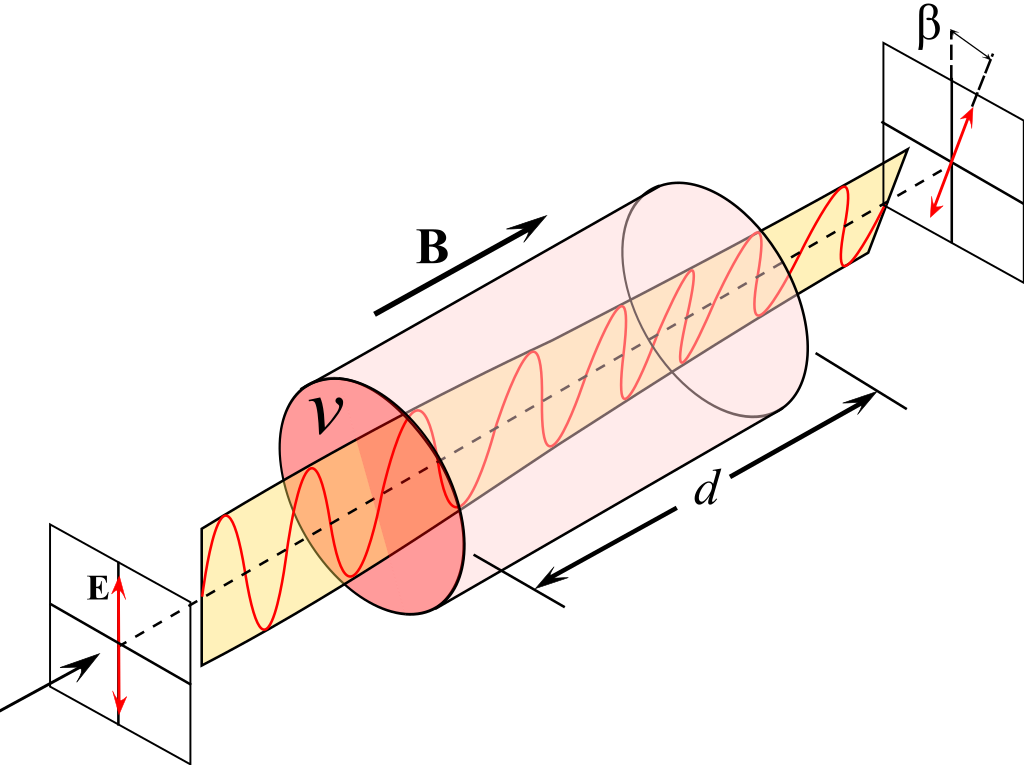
\includegraphics[width=12cm]{fotos/FaradayEffekt.png}
    \caption{Zu sehen ist der Faraday-Effekt. Die rote Linie beschreibt das linear polarisierte Licht. In gelb ist die Polarisationsebene hervorgehoben. Das Medium der Länge $d$ ist rötlich dargestellt. Hier bezeichnet $\beta$ die Drehung der Polarisationsebene. \cite{Faraday}}
    \label{fig:FaradayEffekt}    
\end{figure}

\begin{equation}
    \theta = \frac{\theta_1 - \theta_2}{2L}
\end{equation}